\documentclass[tikz,border=5pt]{standalone}
\usepackage{tikz}
\usepackage{pgfplots}
\usepgfplotslibrary{groupplots}
\pgfplotsset{compat=1.18}
% sha256: e6552abb73343471d8bbd240896ae48f7ab5859a3ba2f667759b9196806e6ff1
\definecolor{p06color0}{HTML}{0072B2}
\definecolor{p06color1}{HTML}{777777}
\begin{document}
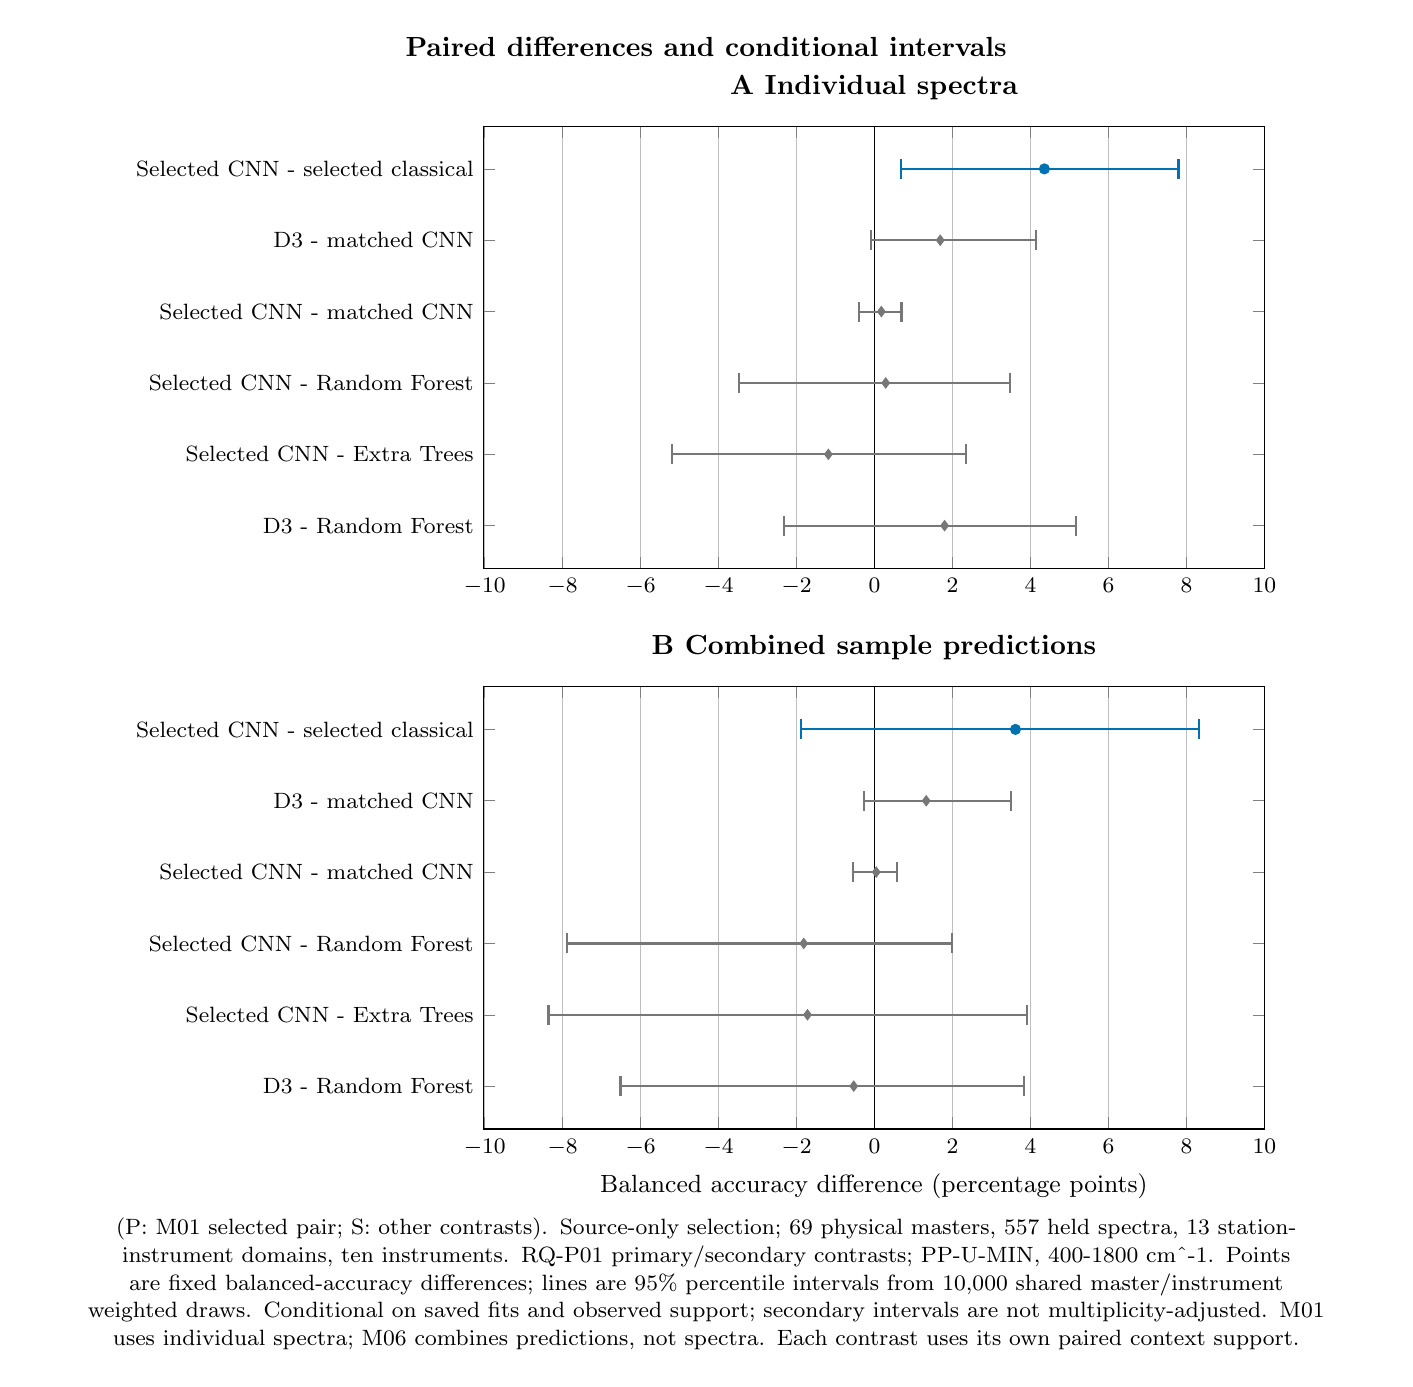
\begin{tikzpicture}
\begin{groupplot}[group style={group size=1 by 2, vertical sep=1.5cm},
width=11.5cm,
height=7.2cm,
xmin=-10.0317607953696, xmax=9.99817906304807,
tick label style={font=\fontsize{8}{10}\selectfont, color=black},
yticklabel style={font=\fontsize{8}{10}\selectfont, color=black},
title style={font=\bfseries\fontsize{10}{12}\selectfont, color=black},
xlabel style={font=\fontsize{9}{11}\selectfont, color=black},
xmajorgrids=true,
ymajorgrids=false]
\nextgroupplot[title={A Individual spectra}, ytick={1,2,3,4,5,6}, yticklabels={D3 - Random Forest,Selected CNN - Extra Trees,Selected CNN - Random Forest,Selected CNN - matched CNN,D3 - matched CNN,Selected CNN - selected classical}, ymin=0.4, ymax=6.6]
\addplot[forget plot, black, thin] coordinates {(0,0.4) (0,6.6)};
\addplot[forget plot, color=p06color1, thick] coordinates {(-2.32377498701124,1) (5.17357340438867,1)};
\addplot[forget plot, color=p06color1, thick] coordinates {(-2.32377498701124,0.86) (-2.32377498701124,1.14)};
\addplot[forget plot, color=p06color1, thick] coordinates {(5.17357340438867,0.86) (5.17357340438867,1.14)};
\addplot[only marks, mark=diamond*, mark size=1.8pt, color=p06color1] coordinates {(1.79530192030192,1)};
\addplot[forget plot, color=p06color1, thick] coordinates {(-5.18811316282539,2) (2.34553624777623,2)};
\addplot[forget plot, color=p06color1, thick] coordinates {(-5.18811316282539,1.86) (-5.18811316282539,2.14)};
\addplot[forget plot, color=p06color1, thick] coordinates {(2.34553624777623,1.86) (2.34553624777623,2.14)};
\addplot[only marks, mark=diamond*, mark size=1.8pt, color=p06color1] coordinates {(-1.18523606023606,2)};
\addplot[forget plot, color=p06color1, thick] coordinates {(-3.48008872899962,3) (3.47395047310304,3)};
\addplot[forget plot, color=p06color1, thick] coordinates {(-3.48008872899962,2.86) (-3.48008872899962,3.14)};
\addplot[forget plot, color=p06color1, thick] coordinates {(3.47395047310304,2.86) (3.47395047310304,3.14)};
\addplot[only marks, mark=diamond*, mark size=1.8pt, color=p06color1] coordinates {(0.28511766011766,3)};
\addplot[forget plot, color=p06color1, thick] coordinates {(-0.397623951002217,4) (0.688504869480541,4)};
\addplot[forget plot, color=p06color1, thick] coordinates {(-0.397623951002217,3.86) (-0.397623951002217,4.14)};
\addplot[forget plot, color=p06color1, thick] coordinates {(0.688504869480541,3.86) (0.688504869480541,4.14)};
\addplot[only marks, mark=diamond*, mark size=1.8pt, color=p06color1] coordinates {(0.173483923483923,4)};
\addplot[forget plot, color=p06color1, thick] coordinates {(-0.0917178002912358,5) (4.13241958831975,5)};
\addplot[forget plot, color=p06color1, thick] coordinates {(-0.0917178002912358,4.86) (-0.0917178002912358,5.14)};
\addplot[forget plot, color=p06color1, thick] coordinates {(4.13241958831975,4.86) (4.13241958831975,5.14)};
\addplot[only marks, mark=diamond*, mark size=1.8pt, color=p06color1] coordinates {(1.68366818366818,5)};
\addplot[forget plot, color=p06color0, thick] coordinates {(0.68373247447679,6) (7.79477318696698,6)};
\addplot[forget plot, color=p06color0, thick] coordinates {(0.68373247447679,5.86) (0.68373247447679,6.14)};
\addplot[forget plot, color=p06color0, thick] coordinates {(7.79477318696698,5.86) (7.79477318696698,6.14)};
\addplot[only marks, mark=*, mark size=1.8pt, color=p06color0] coordinates {(4.35573093248532,6)};
\nextgroupplot[title={B Combined sample predictions}, xlabel={Balanced accuracy difference (percentage points)}, ytick={1,2,3,4,5,6}, yticklabels={D3 - Random Forest,Selected CNN - Extra Trees,Selected CNN - Random Forest,Selected CNN - matched CNN,D3 - matched CNN,Selected CNN - selected classical}, ymin=0.4, ymax=6.6]
\addplot[forget plot, black, thin] coordinates {(0,0.4) (0,6.6)};
\addplot[forget plot, color=p06color1, thick] coordinates {(-6.51806963456126,1) (3.83935038545567,1)};
\addplot[forget plot, color=p06color1, thick] coordinates {(-6.51806963456126,0.86) (-6.51806963456126,1.14)};
\addplot[forget plot, color=p06color1, thick] coordinates {(3.83935038545567,0.86) (3.83935038545567,1.14)};
\addplot[only marks, mark=diamond*, mark size=1.8pt, color=p06color1] coordinates {(-0.534188034188035,1)};
\addplot[forget plot, color=p06color1, thick] coordinates {(-8.36259914050144,2) (3.89921103593014,2)};
\addplot[forget plot, color=p06color1, thick] coordinates {(-8.36259914050144,1.86) (-8.36259914050144,2.14)};
\addplot[forget plot, color=p06color1, thick] coordinates {(3.89921103593014,1.86) (3.89921103593014,2.14)};
\addplot[only marks, mark=diamond*, mark size=1.8pt, color=p06color1] coordinates {(-1.72008547008547,2)};
\addplot[forget plot, color=p06color1, thick] coordinates {(-7.883968265348,3) (1.9890484054175,3)};
\addplot[forget plot, color=p06color1, thick] coordinates {(-7.883968265348,2.86) (-7.883968265348,3.14)};
\addplot[forget plot, color=p06color1, thick] coordinates {(1.9890484054175,2.86) (1.9890484054175,3.14)};
\addplot[only marks, mark=diamond*, mark size=1.8pt, color=p06color1] coordinates {(-1.81623931623932,3)};
\addplot[forget plot, color=p06color1, thick] coordinates {(-0.547940591149345,4) (0.571102239171907,4)};
\addplot[forget plot, color=p06color1, thick] coordinates {(-0.547940591149345,3.86) (-0.547940591149345,4.14)};
\addplot[forget plot, color=p06color1, thick] coordinates {(0.571102239171907,3.86) (0.571102239171907,4.14)};
\addplot[only marks, mark=diamond*, mark size=1.8pt, color=p06color1] coordinates {(0.0427350427350427,4)};
\addplot[forget plot, color=p06color1, thick] coordinates {(-0.261657354061373,5) (3.50365475008811,5)};
\addplot[forget plot, color=p06color1, thick] coordinates {(-0.261657354061373,4.86) (-0.261657354061373,5.14)};
\addplot[forget plot, color=p06color1, thick] coordinates {(3.50365475008811,4.86) (3.50365475008811,5.14)};
\addplot[only marks, mark=diamond*, mark size=1.8pt, color=p06color1] coordinates {(1.32478632478632,5)};
\addplot[forget plot, color=p06color0, thick] coordinates {(-1.88160425998068,6) (8.32901740817993,6)};
\addplot[forget plot, color=p06color0, thick] coordinates {(-1.88160425998068,5.86) (-1.88160425998068,6.14)};
\addplot[forget plot, color=p06color0, thick] coordinates {(8.32901740817993,5.86) (8.32901740817993,6.14)};
\addplot[only marks, mark=*, mark size=1.8pt, color=p06color0] coordinates {(3.61373519268256,6)};
\end{groupplot}
\node[anchor=south, font=\bfseries\fontsize{10}{12}\selectfont] at (current bounding box.north) {Paired differences and conditional intervals};
\node[anchor=north, text width=17cm, align=center, font=\fontsize{8}{10}\selectfont] at (current bounding box.south) {(P: M01 selected pair; S: other contrasts). Source-only selection; 69 physical masters, 557 held spectra, 13 station-instrument domains, ten instruments. RQ-P01 primary/secondary contrasts; PP-U-MIN, 400-1800 cm\textasciicircum{}-1. Points are fixed balanced-accuracy differences; lines are 95\% percentile intervals from 10,000 shared master/instrument weighted draws. Conditional on saved fits and observed support; secondary intervals are not multiplicity-adjusted. M01 uses individual spectra; M06 combines predictions, not spectra. Each contrast uses its own paired context support.};
\end{tikzpicture}
\end{document}
